\documentclass[11pt]{article}
\usepackage[a4paper,margin=0.92in]{geometry}
\usepackage{amsmath,amssymb,amsthm,mathtools}
\usepackage{booktabs,array,graphicx,xcolor,xurl,float,multicol}
\usepackage[hidelinks]{hyperref}
\hypersetup{pdftitle={Projective Memory and Resonant Bottlenecks in Passive Multiport Routing},pdfauthor={Lluis Eriksson},pdfsubject={Exact global state laws, robust error floors, and high-delay border phases}}
\usepackage[nameinlink,capitalise]{cleveref}
\usepackage{microtype,etoolbox}
\AtBeginEnvironment{thebibliography}{\fontsize{8}{9}\selectfont\setlength{\itemsep}{-2pt}\setlength{\parsep}{0pt}}

\newtheorem{theorem}{Theorem}[section]
\newtheorem{lemma}[theorem]{Lemma}
\newtheorem{corollary}[theorem]{Corollary}
\newtheorem{proposition}[theorem]{Proposition}
\theoremstyle{definition}\newtheorem{definition}[theorem]{Definition}\newtheorem{example}[theorem]{Example}
\theoremstyle{remark}\newtheorem{remark}[theorem]{Remark}\newtheorem{limitation}[theorem]{Limitation}
\crefname{lemma}{Lemma}{Lemmas}\crefname{proposition}{Proposition}{Propositions}
\crefname{corollary}{Corollary}{Corollaries}\crefname{limitation}{Limitation}{Limitations}
\crefname{definition}{Definition}{Definitions}\crefname{example}{Example}{Examples}
\crefname{remark}{Remark}{Remarks}
\newcommand{\C}{\mathbb C}\newcommand{\D}{\mathbb D}\newcommand{\T}{\mathbb T}
\newcommand{\PP}{\mathbb P}\newcommand{\rank}{\operatorname{rank}}
\newcommand{\Res}{\operatorname{Res}}\newcommand{\mcdeg}{\deg_{\mathrm{McM}}}
\newcommand{\norm}[1]{\lVert#1\rVert}\newcommand{\dd}{\,\mathrm d}
\newcolumntype{L}[1]{>{\raggedright\arraybackslash}p{#1}}

\title{Projective Memory and Resonant Bottlenecks in Passive Multiport Routing:\\
Exact Global Laws, Robust Error Floors, and High-Delay Border Phases}
\author{Lluis Eriksson}
\date{13 August 2026}

\begin{document}
\maketitle

\begin{abstract}
At distinct boundary frequencies $\zeta_i$, let a square rational-inner
multiport route one fixed input ray to prescribed output rays $Y_i$.  Put
$H=\operatorname{span}(Y_1,\ldots,Y_L)$ and let $\delta_H$ be the least degree
of a base-point-free projective map
$R:\PP^1\to\PP(H)$ satisfying $R(\zeta_i)=Y_i$.  We prove the global identity
\[
                         d_{\min}=\delta_H,
\]
independently of the ambient port count.  A scalar Fej\'er--Riesz factorization
followed by a same-state-dimension rectangular lossless completion proves
attainability.  Conversely, a common realization denominator and the strict
inequality $d_{\min}<L$ force every optimal routed column to lie identically in
$H$, where it becomes a projective interpolant.  This converts the full line-
routing problem into a finite algebraic degree problem and contains the
direct-sum, repeated-target, and coplanar laws as strata.

For orthogonal target bands we solve line-to-subspace incidence constraints.
Full-support Lagrange kernels give every exact degree, while the
generic law is a closed codimension formula.  Exact memory takes the maximum
shifted band cost, whereas border memory takes the minimum; this max--min split
can be arbitrarily large.

For $r=\dim H$, orthonormal annihilators of the targets define an intrinsic
incidence matrix $A_d$ with $L(r-1)$ rows and $r(d+1)$ columns.  Its
minimum modulus gives the calibrated error floor
\[
 E_d\ge \frac{\sigma_{\min}(A_d)}
 {\sqrt{L(d+1)+\sigma_{\min}(A_d)^2}},
\]
stable under operator-norm perturbations.  More sharply,
$E_d=0$ if and only if $A_d$ has a kernel.  Hence border memory obeys both
a linear rank law and the all-data base-point deletion formula
\[
 d_\partial=\min\{d:\ker A_d\ne0\}
 =\min_{B\subseteq[L]}\bigl(|B|+\Delta(B^c)\bigr).
\]
The universal dense-routing threshold is
$\lfloor L(r-1)/r\rfloor$ and is generically sharp.
In the planar stratum the zero-error closure is the determinantal locus cut
out by the maximal minors of $M_d$, and all border degrees are found by one
incremental exact elimination using $O(L^3)$ field operations.

The closure phase has an operational cost.  If
$d_\partial\le d<d_{\min}$, then arbitrarily accurate degree-$d$ routers exist
but every such approximating sequence has divergent peak Wigner--Smith delay,
$\|\operatorname{tr}Q\|_\infty\to\infty$.  Under any finite peak-delay cap the
best error is strictly positive and attained.  Thus the exact trichotomy is
physical as well as algebraic: robust positive-error phase, singular high-delay
border phase, and exact finite-delay phase.  In the planar stratum we additionally
solve degree zero by the smallest Bloch-sphere cap, prove the exact binary
occupancy law, classify all four-node tables by multiplicity and cross-ratio,
and certify a strict $21\%$ one-state error barrier.  Exact artifacts and an
independent verifier accompany the theorem fixtures.  Classical rational
interpolation and lossless completion are credited as ingredients; the result
claimed here is their global state--error--delay synthesis.
\end{abstract}

\noindent\textbf{Keywords:} rational inner matrix; projective interpolation;
McMillan degree; passive memory; border memory; resonant approximation;
chordal error; lossless completion; Wigner--Smith delay.

\section{The global line-routing problem}

Let $S$ be an $N\times N$ rational matrix, analytic in $\D$, unitary almost
everywhere on $\T$, and regular at distinct nodes
$\zeta_1,\ldots,\zeta_L\in\T$.  Its McMillan degree is the state dimension of a
minimal conservative realization.  Fix an input line $X\subset\C^N$ and target
lines $Y_i\subset\C^N$.  The routing task is
\begin{equation}\label{eq:routing}
                              S(\zeta_i)X=Y_i,
                              \qquad 1\le i\le L.
\end{equation}
Endpoint phases and bases are free.  Write $d_{\min}$ for the least McMillan
degree among all such $S$.

Put $H=\operatorname{span}(Y_1,\ldots,Y_L)$ and $r=\dim H$.  Earlier exact
occupancy laws cover direct-sum target families and give detector lower bounds
on singular arrangements \cite{ErikssonUnified2026}.  They do not give an
equality theory for an arbitrary line table.  The point of the present paper is
that for one input line the missing invariant is the degree of a projective
curve through the ordered data.  Taking $H$ to be the actual target span makes
the resulting theorem global, not a fixed-rank special case.

Classical scalar, matrix, and tangential rational interpolation and their
state-variable realizations describe minimal rational functions through finite
data \cite{AntoulasAnderson1986,AndersonAntoulas1990,AntoulasEtAl1990,Ravi1997,CortadellasEtAl2020}.
Minimal boundary interpolation by scalar unimodular functions and finite
Blaschke products is also well developed
\cite{Glader2006,SemmlerWegert2006,Bolotnikov2018}.  Subspace Nevanlinna
interpolation and boundary matrix all-pass construction provide the matrix
context \cite{RapisardaWillems1997,BolotnikovDym2006,BharathEtAl2023}.
Rectangular lossless realization and same-state square completion are likewise
classical \cite{AlpayJorgensenLewkowicz2016}.  Our contribution is not a new
rational interpolation algorithm or a new completion theorem.  It is the
global identification of projective interpolation degree with passive state
count, together with an intrinsic quantitative error operator, the exact
border-memory law, and the divergent peak-delay theorem for every nonattained
border phase.  The complete planar and four-line classifications then become
explicit singular strata of the global result.

The rank formula is the computational hinge.  Exact memory asks whether a
kernel vector polynomial is primitive and base-point-free, a nonlinear common-
zero condition; border memory asks only whether a nonzero kernel vector exists.
This separates exact realization from closure by one algebraic operation and
turns the sign question for $E_d$ into linear algebra.

\begin{table}[t]
\centering
\small
\caption{Classical interfaces and the paper-specific deductions.  The first
two columns are not claimed as new.}
\label{tab:known-new}
\begin{tabular}{L{0.23\textwidth}L{0.29\textwidth}L{0.39\textwidth}}
\toprule
Classical interface & What it supplies & Deduction established here\\
\midrule
Minimal rational interpolation
\cite{AntoulasEtAl1990,Ravi1997}
& Rational/projective interpolants through finite data
& Equality of projective degree and passive McMillan state count for every
one-line routing table\\
Rectangular lossless completion
\cite{AlpayJorgensenLewkowicz2016}
& Same-state square para-unitary completion
& Exact lossless compiler attaining the projective lower bound in the ambient
multiport\\
Base points and unattainable data
\cite{Glader2008,CortadellasUnattainable2018}
& Common-factor and nonattainment mechanisms
& Rank/error dichotomy, deletion law, determinantal closure, and the exact
versus border max--min split\\
Potapov factors and group delay
\cite{Potapov1955,Wigner1955,Smith1960}
& Factorization, winding and Poisson delay kernels
& Divergent peak delay forced along every nonattained zero-error routing
sequence\\
\bottomrule
\end{tabular}
\end{table}

\section{Projective degree equals passive memory in every dimension}

A vector polynomial $p=(p_1,\ldots,p_r)^T$ is \emph{primitive} if its
coordinates have no common projective zero, including at infinity.  It then
defines a morphism $[p]:\PP^1\to\PP(H)$ whose degree is the maximum coordinate
degree after removal of the common homogeneous factor.

\begin{definition}[Global projective interpolation degree]\label{def:global-delta}
Let
\[
 \delta_H=\min\{\deg R:R:\PP^1\to\PP(H),\quad
                         R(\zeta_i)=Y_i\ (1\le i\le L)\}.
\]
For a subtable $A\subseteq[L]$ we write $\delta_H(A)$ for the same minimum on
$A$, with $\delta_H(\varnothing)=0$.
\end{definition}

\begin{lemma}[Exact-state lossless compiler]\label{lem:lossless-compiler}
Let $p=(p_1,\ldots,p_r)^T$ be a primitive polynomial vector of projective
degree $\delta$.  Then there is an $r\times r$ rational-inner matrix $S_p$ and
a constant input vector $u$ such that $S_pu$ represents $[p]$ and
\[
 \deg p_a\le\delta,\qquad \deg h\le\delta,\qquad
 \mcdeg(p/h)=\mcdeg S_p=\delta,
\]
where $h$ is outer and $|h|^2=\sum_a|p_a|^2$ on $\T$.
\end{lemma}

\begin{proof}
The positive Laurent polynomial $\sum_a|p_a|^2$ has bandwidth at most
$\delta$.  Scalar Fej\'er--Riesz factorization therefore supplies an outer
spectral factor $h$ of degree at most $\delta$, so $f=p/h$ is an inner
$r\times1$ column with at most $\delta$ states.  If $f$ admitted an $n$-state
realization with $n<\delta$, clearing its common realization denominator would
produce a polynomial projective representative of degree at most $n$, contrary
to the minimal projective degree of $[p]$.  Hence $\mcdeg f=\delta$.

The completion interface is used with its convention made explicit.  The
function $f$ is analytic in $\D$ and isometric on $\T$; reflect it to the
exterior-disk coisometric row
$f^\sharp(z)=f(1/\bar z)^*$.  The minimal realization completion
\cite[Theorem~2.1(ii)]{AlpayJorgensenLewkowicz2016} extends $f^\sharp$ to a
square para-unitary matrix with the same state dimension.  Reflection back,
followed by constant unitary changes of input and output bases, gives $S_p$
without adding states.
\end{proof}

\begin{theorem}[Global projective memory law]\label{thm:global}
For every finite line-routing table at distinct boundary nodes,
\begin{equation}\label{eq:global}
                         \boxed{d_{\min}=\delta_H.}
\end{equation}
The equality is independent of the ambient port number.  A minimum-degree
projective interpolant compiles to a square lossless router of the same degree.
\end{theorem}

\begin{proof}
Vector Lagrange interpolation gives $\delta_H\le L-1$.  Choose a primitive
polynomial representative $p=(p_1,\ldots,p_r)^T$ of a minimum interpolant,
all coordinates padded to degree $\delta_H$.  Lemma~\ref{lem:lossless-compiler}
compiles it to a square rational-inner router of exactly the same state
dimension.  An identity block embeds it in the ambient port space, proving
$d_{\min}\le\delta_H$.

Conversely let $S$ be a minimum-degree router, $d=\mcdeg S$.  The upper bound
gives $d\le L-1<L$.  For a unit vector $x$ spanning the input line, a stable
minimal realization writes the routed column as $F=Sx=n/\chi$, where every
coordinate of the vector polynomial $n$ and the common denominator $\chi$ has
degree at most $d$, and $\chi(\zeta_i)\ne0$.  If $\ell$ annihilates $H$, then
$\ell n$ vanishes at all $L>d$ nodes, so $\ell n\equiv0$.  Thus $F$ takes
values identically in $H$.  Cancel the common homogeneous factor from its $r$
coordinate numerators.  The resulting primitive projective map has degree at
most $d$ and interpolates every $Y_i$.  Therefore $\delta_H\le d$.
\end{proof}

\begin{corollary}[Span and direct-sum strata]\label{cor:global-strata}
Every table satisfies $\delta_H\ge r-1$.  If the $L$ targets are linearly
independent, then $r=L$ and $d_{\min}=L-1$.  For $r=2$ the global invariant is
the ordinary rational-map degree on $\PP^1$ developed below.
\end{corollary}

\begin{proof}
The image of a degree-$d$ map $\PP^1\to\PP(H)$ spans projective dimension at
most $d$, because it is the linear projection of the degree-$d$ Veronese
curve.  Hence $d\ge r-1$.  For independent targets, Lagrange interpolation
gives the reverse bound $L-1$.
\end{proof}

\section{Block-subspace interpolation and full-support kernels}

The line law admits a nontrivial incidence extension.  Let
\[
 H=H_1\oplus\cdots\oplus H_B,\qquad \dim H_b=r_b,
\]
and partition the nodes into nonempty sets $I_b$, $|I_b|=L_b$.  At a node
$i\in I_b$, prescribe a nonzero subspace $Y_i\subseteq H_b$ of dimension
$s_i$.  The routed output is still one line, but it may be chosen freely in
$\PP(Y_i)$.  Let $\Delta(J)$ be the least degree of a base-point-free vector
polynomial satisfying the records in $J\subseteq[L]$, and set
$\Delta(\varnothing)=0$.  Write $\Delta=\Delta([L])$; equivalently, $\Delta$
is the least degree of a base-point-free vector
polynomial $F$ satisfying
\begin{equation}\label{eq:incidence}
                         F(\zeta_i)\in Y_i\setminus\{0\}.
\end{equation}
The proof of Theorem~\ref{thm:global}, with line equality replaced by
incidence, gives $d_{\min}=\Delta$.

For each block, let $\ell_{b,i}$ be the scalar Lagrange polynomial on the
nodes in $I_b$.  If $0\le q\le L_b-1$, define
\[
 T_{b,q}:\bigoplus_{i\in I_b}Y_i\longrightarrow H_b\otimes\C^q
\]
by taking the top $q$ coefficient vectors of
$\sum_{i\in I_b}\ell_{b,i}(z)u_i$.  Put
\begin{equation}\label{eq:qstar}
 q_b^*=\max\{q:\ker T_{b,q}\text{ contains }(u_i)_{i\in I_b}
                       \text{ with every }u_i\ne0\}.
\end{equation}
The full-support clause in \eqref{eq:qstar} is essential: an ordinary kernel
may silently delete a record.

\begin{lemma}[Hall--Vandermonde assignment]\label{lem:hall-vandermonde}
Fix distinct nodes, $r$ coordinate blocks, row demands
$0\le c_i\le r$, and $C=\sum_i c_i$.  For polynomials of degree at most $e$,
there is a choice of coordinate quotient spaces of dimensions $c_i$ whose
incidence matrix has rank
\[
                         \min\{C,r(e+1)\}.
\]
Consequently maximal rank holds on a Zariski-open dense set of quotient
spaces with the same dimensions.
\end{lemma}

\begin{proof}
View the $c_i$ restrictions at node $i$ as edges from that node to distinct
coordinate blocks.  If $C\le r(e+1)$, seek a $0$--$1$ assignment with row
sums $c_i$ and column sums at most $e+1$.  Hall's capacitated condition holds:
for a node subset $J$ with $|J|\le e+1$ its demand is at most $r|J|$, while
for $|J|>e+1$ it is at most $C\le r(e+1)$.  The assigned evaluation rows split
into coordinate Vandermonde blocks of at most $e+1$ rows, so they are linearly
independent and the incidence matrix has full row rank.

If $C\ge r(e+1)$, first assign $e+1$ rows to every coordinate, using at most
$c_i$ rows at node $i$.  For any set of $k$ coordinates,
\[
 \sum_i\min\{c_i,k\}\ge \frac{k}{r}\sum_i c_i\ge k(e+1),
\]
which is the dual Hall condition.  Fill the remaining row demands arbitrarily.
Each coordinate now contains an invertible $(e+1)\times(e+1)$ Vandermonde
block, giving full column rank.  In either case a maximal minor is nonzero for
one coordinate configuration.  Since that minor is polynomial in local
Grassmannian coordinates, its nonvanishing locus is Zariski open and dense.
\end{proof}

\begin{theorem}[Exact full-support block law]\label{thm:block}
Every block-subspace table satisfies
\begin{equation}\label{eq:block}
 \boxed{\quad d_{\min}=\Delta
 =\max_b\{L-L_b+L_b-1-q_b^*\}
 =L-1-\min_b q_b^*.\quad}
\end{equation}
For fixed dimensions $(r_b,s_i)$, on a Zariski-open dense set of target
subspaces,
\begin{equation}\label{eq:block-generic}
 d_{\min}^{\rm gen}
 =\max_b\left\{L-L_b+\left\lfloor
             \frac{\sum_{i\in I_b}(r_b-s_i)}{r_b}\right\rfloor\right\}.
\end{equation}
For one $r$-dimensional block of line targets this becomes
\begin{equation}\label{eq:global-generic}
                     d_{\min}^{\rm gen}
                     =\left\lfloor\frac{L(r-1)}r\right\rfloor.
\end{equation}
\end{theorem}

\begin{proof}
Write $F=(F_b)_b$.  At every node outside $I_b$, the component $F_b$ must
vanish.  Hence
\[
 F_b(z)=Z_{\neg b}(z)G_b(z),\qquad
 Z_{\neg b}(z)=\prod_{i\notin I_b}(z-\zeta_i).
\]
On $I_b$ the scalar factor is nonzero.  The unique polynomial $G_b$ of degree
at most $L_b-1$ with chosen values $u_i\in Y_i$ is their Lagrange sum.  It
loses its top $q$ coefficients precisely when $(u_i)\in\ker T_{b,q}$, and it
serves every node precisely when all $u_i$ are nonzero.  At the maximal $q$
it is primitive: division by a common scalar factor would preserve the
nonzero node values and produce one additional vanished leading coefficient.
The forced factor has degree $L-L_b$; simultaneous service of every block
takes the maximum shifted degree.  The global vector has no base point: its
own block is nonzero at each record; away from all records every block is
nonzero; and at infinity a maximum-degree block has nonzero leading vector.
This proves \eqref{eq:block}.  A full-support
kernel exists exactly when no coordinate projection of $\ker T_{b,q}$ is
zero, since finitely many proper linear subspaces cannot cover a complex
vector space.

For genericity consider the incidence map at intrinsic degree $e$,
\[
 A_{b,e}:H_b\otimes\C[z]_{\le e}\longrightarrow
                \bigoplus_{i\in I_b}H_b/Y_i.
\]
Its generic rank is the smaller of its $r_b(e+1)$ columns and
$C_b=\sum_i(r_b-s_i)$ rows by Lemma~\ref{lem:hall-vandermonde}.  The first generic kernel therefore occurs at
$e=\lfloor C_b/r_b\rfloor$.  There its dimension is
$k=r_b(e+1)-C_b\in\{1,\ldots,r_b\}$, whereas the kernel subspace vanishing at
node $i$ has generic dimension $\max\{0,k-s_i\}<k$.  The finite
union of these exceptional subspaces is not the whole kernel.  The first
full-support vector is primitive, or division would contradict minimality of
$e$.  Adding the forced shifts and taking the maximum proves
\eqref{eq:block-generic}; \eqref{eq:global-generic} is its one-block line
specialization.
\end{proof}

For a fixed total line-record budget $L$, nonempty bands of dimensions $r_b$,
and $R=\sum_b r_b$, optimizing the allocation gives the exact generic design
law
\begin{equation}\label{eq:allocation}
 d_{\rm opt}=L-1-\left\lfloor\frac{L-B}{R}\right\rfloor.
\end{equation}
It is attained whenever
$L_b\ge r_b\lfloor(L-B)/R\rfloor+1$ for every $b$; residual records may be
assigned arbitrarily.

\section{Incidence rank, robust error, and border memory}

Choose for each $Y_i$ an orthogonal quotient map
$Q_i:H\to H\ominus Y_i$.  On coefficient vectors of $H$-valued polynomials
of degree at most $d$, define the intrinsic incidence matrix
\begin{equation}\label{eq:Ad}
 A_d c=\bigl(Q_i p_c(\zeta_i)\bigr)_{i=1}^L.
\end{equation}
Unitary basis changes do not change its singular values.  Let $E_d$ be the
infimum worst-node chordal distance to the prescribed projective subspaces.

\begin{theorem}[Rank--error dichotomy and base-point deletion]\label{thm:global-border}
For every incidence table,
\begin{align}
 E_d=0&\quad\Longleftrightarrow\quad\ker A_d\ne\{0\},
                                                        \label{eq:rank-border}\\
 d_\partial:=\min\{d:E_d=0\}
 &=\min_{B_0\subseteq[L]}\bigl\{|B_0|+\Delta(B_0^c)\bigr\}.
                                                        \label{eq:delete}
\end{align}
If $A_d$ has full column rank and $\sigma_d=\sigma_{\min}(A_d)>0$, then
\begin{equation}\label{eq:global-error}
 E_d\ge\boxed{\frac{\sigma_d}
                    {\sqrt{L(d+1)+\sigma_d^2}}}.
\end{equation}
If normalized data perturb $A_d$ by operator norm at most $\eta<\sigma_d$,
the same bound holds with $\sigma_d$ replaced by $\sigma_d-\eta$.

In the block architecture of Theorem~\ref{thm:block}, write
\[
 \bar e_b=\min\{e:\ker A_{b,e}\ne0\}.
\]
Then
\begin{equation}\label{eq:border-min}
 d_\partial=\min_b\{L-L_b+\bar e_b\},
\end{equation}
and generically
\begin{equation}\label{eq:border-generic}
 d_\partial^{\rm gen}=\min_b\left\{L-L_b+\left\lfloor
              \frac{\sum_{i\in I_b}(r_b-s_i)}{r_b}\right\rfloor\right\}.
\end{equation}
Thus exact and border memory use, respectively, the maximum and minimum of the
shifted block costs.
\end{theorem}

\begin{proof}
If a router sequence has errors tending to zero, normalize the coefficients of
the projected numerator and take a convergent subsequence.  Quotient residuals
converge to zero, producing a nonzero element of $\ker A_d$.  Conversely take
$0\ne p\in\ker A_d$, let $B_0$ be the nodes where all coordinates vanish, and
remove its scalar gcd.  The reduced vector serves $B_0^c$ and gives
$|B_0|+\Delta(B_0^c)\le d$.

For the reverse construction put $b=|B_0|$,
$D=b+\Delta(B_0^c)$, choose a primitive minimum interpolant $R$ of $B_0^c$,
and set $P_0=gR$ with
$g(z)=\prod_{i\in B_0}(z-\zeta_i)$.  The cases $B_0=\varnothing$ and
$\dim H=1$ are immediate.  Otherwise choose a functional $\lambda$ nonzero
on every $Y_i$, $i\in B_0$, representatives $a_i\in Y_i$ with
$\lambda(a_i)=1$, and their degree-at-most-$(b-1)$ Lagrange interpolant
$A_0$.  Then $\lambda(A_0)\equiv1$.  For $0\ne v\in\ker\lambda$, the vector
polynomial
\[
                         A(z)=A_0(z)+g(z)z^{D-b}v
\]
has exact degree $D$, serves $B_0$, has no finite base point because
$\lambda(A)\equiv1$, and has nonzero leading vector at infinity.  Thus the
projective pencil $P_0+tA$ is not contained in the common-root locus: its
point at $t=\infty$ is primitive.  Properness of $\PP^1$ makes the exceptional
parameter set algebraic and finite.  Choose nonzero $t_n\to0$ outside it and
also outside the single possible leading-cancellation value.  The primitive
degree-$D$ maps $[P_0+t_nA]$ serve $B_0$ exactly and converge to the required
targets on $B_0^c$.  Lossless completion proves
\eqref{eq:rank-border}--\eqref{eq:delete}.

For \eqref{eq:global-error}, write a routed unit column as $n/\chi$ and let
$c$ be the coefficients of its projection to $H$.  If $\epsilon$ is the
largest node error, orthogonal projection gives
\[
 \|Q_i p_c(\zeta_i)\|\le|\chi(\zeta_i)|\epsilon,
 \qquad
 \|p_c(\zeta_i)\|\ge|\chi(\zeta_i)|\sqrt{1-\epsilon^2}.
\]
Degree-$d$ evaluation on $\T$ has norm $\sqrt{d+1}$.  Summing and comparing
$\|A_dc\|\ge\sigma_d\|c\|$ yields \eqref{eq:global-error}; Weyl's inequality
gives the perturbation statement.  Finally, a global block kernel may live in
one component only, so the first rank loss takes the minimum shifted block
cost, proving \eqref{eq:border-min}--\eqref{eq:border-generic}.
\end{proof}

For two scalar bands with occupancies $(2,4)$, the shifted costs are $(4,2)$.
Hence $d_{\min}=4$ but $d_\partial=2$.  This exact fixture prevents the tempting
but false assertion that generic exact and border memory always coincide.

\begin{figure}[t]
\centering
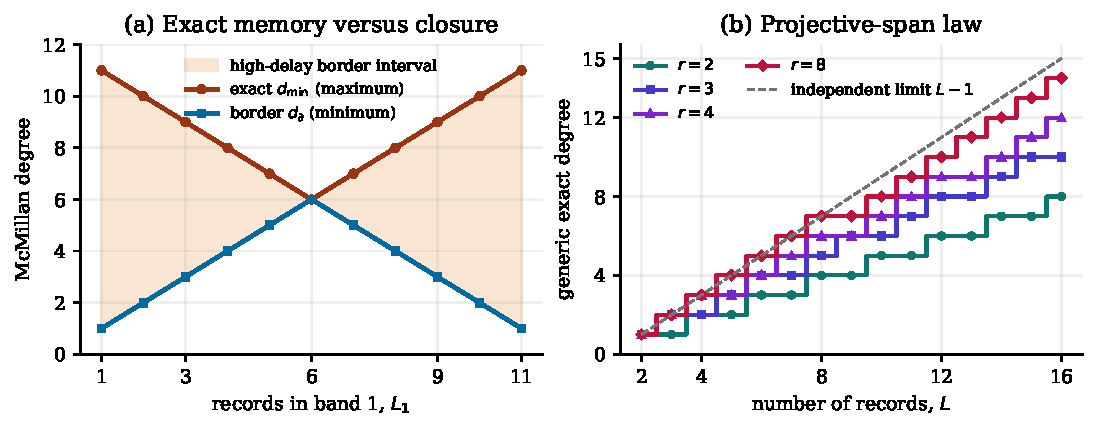
\includegraphics[width=\textwidth]{figures/global_projective_phases.pdf}
\caption{Two consequences of the global laws.  (a) For two scalar bands with
$L=12$, exact memory is the maximum forced-zero count while border memory is
the minimum; the shaded degrees are zero-error but nonattained and therefore
      high-delay.  (b) For one $r$-dimensional target span, generic exact memory is
$\lfloor L(r-1)/r\rfloor$ and approaches the independent-target limit as $r$
grows.  Both panels plot theorem values, not fitted numerics.}
\label{fig:global-phases}
\end{figure}

\begin{table}[t]
\centering
\small
\caption{Exact rational fixtures independently replayed with the manuscript.}
\label{tab:global-fixtures}
\begin{tabular}{L{0.33\textwidth}ccc}
\toprule
Table & $d_\partial$ & $d_{\min}$ & certificate\\
\midrule
$\C^3$ subspaces of dimensions $(2,1,2)$ & 1 & 1 & $\rank A_0=3=\#\mathrm{col}$, $\rank A_1=4<6$\\
Planar four-node $3+1$ collision & 1 & 3 & full-support loss\\
$\C^3$ targets $(2,1,2)\oplus$ two distinct $\C^2$ lines & 3 & 4 & shifted costs $(3,4)$\\
Two scalar bands, occupancies $(2,4)$ & 2 & 4 & $\rank A_1=4=\#\mathrm{col}$, $\rank A_2=5<6$\\
\bottomrule
\end{tabular}
\end{table}

\section{The nonattained phase is necessarily high-delay}

For a differentiable lossless boundary response set
\[
 Q_S(\theta)=-iS(e^{i\theta})^*\frac{d}{d\theta}S(e^{i\theta}),
 \qquad D(S)=\|\operatorname{tr}Q_S\|_\infty.
\]
Let $E_{d,T}$ be the infimum node error among routers with
$\mcdeg S\le d$ and $D(S)\le T$.

\begin{theorem}[Resonant border trichotomy]\label{thm:highq}
For every finite incidence table:
\begin{enumerate}
 \item if $d<d_\partial$, then $E_d>0$, with the explicit floor
       \eqref{eq:global-error} whenever $A_d$ has full column rank;
 \item if $d_\partial\le d<d_{\min}$, then $E_d=0$ but
       $E_{d,T}>0$ for every finite $T$, and every sequence with errors tending
       to zero satisfies $D(S_n)\to\infty$;
 \item if $d\ge d_{\min}$, exact routing is attained by a finite-delay router.
\end{enumerate}
For fixed $d,T$, the constrained minimum defining $E_{d,T}$ is attained.
\end{theorem}

\begin{proof}
A degree-at-most-$d$ rational inner matrix has a rank-one
Blaschke--Potapov factorization \cite{Potapov1955,AlpayJorgensenLewkowicz2016}
\[
 S(z)=\prod_{j=1}^m\left[I+(b_{\alpha_j}(z)-1)v_jv_j^*\right]U,
 \qquad m\le d,
\]
where $U$ is unitary,
$b_\alpha(z)=(z-\alpha)/(1-\bar\alpha z)$, and $\alpha_j\in\D$.
Because the determinant is a constant phase times $\prod_jb_{\alpha_j}$,
Jacobi's formula makes the trace delay the sum of nonnegative Poisson kernels,
\[
 \operatorname{tr}Q_S(\theta)=\sum_{j=1}^m
 \frac{1-|\alpha_j|^2}{|e^{i\theta}-\alpha_j|^2}.
\]
The $j$th summand peaks at $(1+|\alpha_j|)/(1-|\alpha_j|)$.  A finite delay cap
therefore confines all zeros to a compact subdisk.  The directions $v_j$ and
$U$ also lie in compact spaces.  For each $m=0,\ldots,d$ the resulting
parameter space is compact, and the capped degree-at-most-$d$ class is the
finite union of their continuous images.
Thus the capped family is compact and evaluation at the fixed nodes is
continuous.  Its error minimum is attained.

If a capped sequence in the middle phase had errors tending to zero, a
convergent subsequence would yield an exact router of degree at most $d$,
contradicting $d<d_{\min}$.  Hence every zero-error approximating sequence has
unbounded $D(S_n)$; in fact the argument applies to every subsequence, so
$D(S_n)\to\infty$.  The remaining statements follow from
Theorems~\ref{thm:global} and \ref{thm:global-border}.
\end{proof}

Theorem~\ref{thm:highq} turns algebraic nonattainment into an operational
statement: a missing state can be approached only by a resonance whose peak
dimensionless Wigner--Smith delay diverges.  It does not assert an energy,
resonator quality factor, linewidth, loss, or fabrication-cost law.

\section{The planar stratum and its explicit lossless lift}

Choose a basis of $H$ and identify its lines with $\PP(H)\simeq\PP^1$.  A
rational map $R:\PP^1\to\PP^1$ is represented by a coprime polynomial pair
$[p:q]$, and $\deg R=\max(\deg p,\deg q)$.  Poles of the affine ratio $p/q$ are
ordinary points of the projective map, not physical singularities.

\begin{definition}[Projective interpolation degree]\label{def:delta}
For the ordered data $(\zeta_i,Y_i)$, let
\[
 \delta=\min\{\deg R:R:\PP^1\to\PP(H),\ R(\zeta_i)=Y_i\text{ for every }i\}.
\]
\end{definition}

\paragraph{Common-denominator lemma.}
Let $S$ be a rational-inner matrix of McMillan degree at most $d$, and let
$F=Sx$ be any routed column.  There are a polynomial $\chi$ and vector
polynomial $n$ such that
\[
                         F(z)=\frac{n(z)}{\chi(z)},
 \qquad \deg\chi\le d,\qquad \deg n_j\le d.
\]
The denominator can be chosen nonzero at every regular interpolation node.
Indeed, take a stable minimal realization
$S(z)=D+zC(I-zA)^{-1}B$ of dimension at most $d$.  With
$\chi(z)=\det(I-zA)$, the adjugate formula gives the stated degree bounds for
every entry of $Sx$.  Stability makes $\chi$ zero-free on $\overline\D$; more
generally, after cancelling any removable common factor, it is nonzero at each
node where $S$ is regular.

\begin{theorem}[Exact planar reduction]\label{thm:planar}
If all target lines in \eqref{eq:routing} lie in one two-plane $H$, then
\begin{equation}\label{eq:main}
                            \boxed{d_{\min}=\delta.}
\end{equation}
The equality is independent of the ambient dimension and is constructive.
\end{theorem}

\begin{proof}
We first note that $\delta\le L-1$.  Apply a projective change of target chart
whose point at infinity avoids the finite target set, interpolate the resulting
affine values by a polynomial of degree at most $L-1$, and undo the chart.

For the upper bound, let $[p:q]$ be a coprime representative of degree
$\delta$.  For a polynomial $r$ of degree at most $\delta$, set
\[
                   r^\sharp(z)=z^\delta\overline{r(1/\bar z)}.
\]
Because $p$ and $q$ are coprime, they have no common zero; in particular
$|p|^2+|q|^2>0$ on $\T$.  Scalar Fej\'er--Riesz factorization
\cite{DritschelRovnyak2010} supplies an outer polynomial $h$, zero-free
in $\D$, such that on $\T$
\[
                       |h|^2=|p|^2+|q|^2.
\]
Equivalently, $h^\sharp h=p^\sharp p+q^\sharp q$.  Therefore
\begin{equation}\label{eq:completion}
 S_2(z)=\frac1{h(z)}
 \begin{pmatrix}p(z)&-q^\sharp(z)\\q(z)&p^\sharp(z)\end{pmatrix}
\end{equation}
is analytic in $\D$ and unitary on $\T$.  Its first column represents $[p:q]$,
and
\[
                   \det S_2=h^\sharp/h.
\]
The strict positivity above also gives $h(\zeta_i)\ne0$ at every routing node.
With reversal taken at the displayed order $\delta$, the scalar Blaschke
product $h^\sharp/h$ has degree exactly $\delta$; if $\deg h<\delta$, the
missing reversed zeros occur at zero.
For a rational-inner matrix the determinant winding equals its McMillan degree
\cite{Potapov1955}, so $\mcdeg S_2=\delta$.  Constant unitaries align the input
line and the basis of $H$, while a block identity embeds $S_2$ into dimension
$N$ without adding states.  Hence $d_{\min}\le\delta$.

Conversely, take a minimum-degree interpolant $S$ with degree $d$.  The upper
construction already gives $d\le L-1<L$.  A stable conservative realization of
$S$ and the common-denominator lemma above give every entry of the routed column
$F=Sx$ a common denominator of degree at most $d$, nonzero at the boundary
nodes; the corresponding numerators have degree at most $d$.  For every linear functional
$\ell$ annihilating $H$, the numerator of $\ell F$ vanishes at all $L>d$
distinct nodes.  It is therefore zero identically.  Thus $F(z)\in H$ as a
rational identity.  In a basis of $H$, cancel the common polynomial factor of
the two coordinate numerators of $F$.  The resulting coprime pair has degree at
most $d$ and interpolates every $Y_i$, so $\delta\le d$.  This proves
\eqref{eq:main}.
\end{proof}

\begin{remark}[Affine poles are harmless]
The datum $R(z)=1/z$ has an affine pole at zero, but the projective pair $[1:z]$
is regular there.  Formula \eqref{eq:completion} lifts this pair to an analytic
inner column.  Accordingly, pole tests on a chosen affine ratio cannot replace
projective coprimality and Fej\'er--Riesz lifting.
\end{remark}

\section{Exact certificates and quantitative approximation barriers}

Write $Y_i=[a_i:b_i]$ in the chosen basis of $H$.  For $d\ge0$, define the
$L\times2(d+1)$ matrix
\begin{equation}\label{eq:Md}
 M_d(i,:)=
 \bigl(b_i,b_i\zeta_i,\ldots,b_i\zeta_i^d,
       -a_i,-a_i\zeta_i,\ldots,-a_i\zeta_i^d\bigr).
\end{equation}
A coefficient vector in $\ker M_d$ is exactly a polynomial pair $(p,q)$ of
degree at most $d$ satisfying $[p(\zeta_i):q(\zeta_i)]=[a_i:b_i]$, provided it
has no base point at a node.
Multiplying a homogeneous target representative by a nonzero scalar rescales
one row, while changing the basis of $H$ acts by an invertible block change on
the coefficient columns.  Hence every rank condition below is intrinsic to the
ordered projective data.

\begin{proposition}[The planar matrix is the intrinsic incidence operator]
\label{prop:A-equals-M}
For normalized line representatives $y_i=(a_i,b_i)^T$, choose the unit
annihilator $q_i=(-\overline b_i,\overline a_i)^T$ in
\eqref{eq:Ad}.  In the monomial coefficient basis, $A_d$ is $M_d$ up to a
diagonal unitary change of quotient coordinates and an inessential row sign.
Consequently their ranks and singular values agree.  Thus the planar results
below are coordinate realizations of the global rank--error theory, rather
than a second independent reduction.
\end{proposition}

\begin{proof}
The quotient functional $q_i^*$ sends $(p(\zeta_i),q(\zeta_i))^T$ to
$-b_ip(\zeta_i)+a_iq(\zeta_i)$, the negative of row $i$ of
\eqref{eq:Md}.  Changing the phase of $q_i$ only multiplies that row by a
unit scalar.
\end{proof}

\begin{proposition}[Fail-closed degree certificate]\label{prop:certificate}
The number $\delta$ is the least $d$ for which $\ker M_d$ contains a pair
$(p,q)$ generating the unit ideal, equivalently $\gcd(p,q)=1$.  For a
nonconstant pair this can be certified by $\Res(p,q)\ne0$; constant pairs are
checked directly.  Such a pair is an exact upper certificate.
Full column rank of $M_{d-1}$ is an exact lower certificate.
\end{proposition}

\begin{proof}
The unit-ideal condition is precisely projective coprimality.  When both
polynomials form a nonconstant pair, it is equivalent to nonvanishing of the
resultant; the constant pairs $[c:0]$ and $[0:c]$, $c\ne0$, are checked by the
unit-ideal condition itself.  The claim follows from Definition~\ref{def:delta} and
\eqref{eq:Md}.  Full column rank excludes every nonzero pair of degree at most
$d-1$.
\end{proof}

The formulation is deliberately algebraic.  A kernel vector alone is not
enough: a common factor can inflate its displayed degree or introduce a base
point.  A B\'ezout identity $up+vq=1$ is an equivalent independently checkable
coprimality certificate.

We now normalize $(a_i,b_i)$ to unit norm and choose an orthonormal basis of
$H$.  For a unit vector $u$ and a target line $Y=\C y$, $\norm y=1$, write
\[
 \operatorname{dist}_{\rm ch}(\C u,Y)
 =\sqrt{1-|\langle u,y\rangle|^2}
\]
for complex-projective chordal distance.

\begin{theorem}[Quantitative approximate-routing obstruction]\label{thm:approx}
Suppose $M_d$ has full column rank and put
$\sigma=\sigma_{\min}(M_d)>0$.  Every square rational-inner router $S$ of
McMillan degree at most $d$ satisfies
\begin{equation}\label{eq:approx}
 \max_{1\le i\le L}\operatorname{dist}_{\rm ch}
       \bigl(S(\zeta_i)X,Y_i\bigr)
 \ \ge\ \boxed{\frac{\sigma}{\sqrt{L(d+1)+\sigma^2}}}.
\end{equation}
If a perturbed normalized data matrix $\widehat M_d$ obeys
$\norm{\widehat M_d-M_d}_2\le\eta<\sigma$, the right-hand side remains valid
with $\sigma$ replaced by $\sigma-\eta$.
Equivalently, the degree-constrained minimax error
$E_d=\inf_{\mcdeg S\le d}\max_i\operatorname{dist}_{\rm ch}(S(\zeta_i)X,Y_i)$
obeys the same lower bound.
\end{theorem}

\begin{proof}
Choose a unit input vector $x$ and write $F=Sx$.  On $\T$, $\norm{F}=1$.
By the common-denominator lemma above, the two coordinates of $P_HF$ have the form
$p/\chi,q/\chi$, with numerator degrees at most $d$.  Let $c$ collect their
$2(d+1)$ coefficients.  If $c=0$, then $F$ is orthogonal to every $Y_i$ and
the left-hand side of \eqref{eq:approx} is one, so assume $c\ne0$.

Put $v_i=(p(\zeta_i),q(\zeta_i))$ and
$e_i=\operatorname{dist}_{\rm ch}(\C F(\zeta_i),Y_i)$.  Since
$v_i=\chi(\zeta_i)P_HF(\zeta_i)$ and $y_i\in H$, the two-dimensional wedge
identity gives
\[
 |(M_dc)_i|=|\det(y_i,v_i)|\le |\chi(\zeta_i)|e_i,
 \qquad
 \norm{v_i}\ge |\chi(\zeta_i)|\sqrt{1-e_i^2}.
\]
Evaluation of two degree-$d$ polynomials at a unit-modulus node has operator
norm $\sqrt{d+1}$, hence $\norm{v_i}\le\sqrt{d+1}\norm c$.  If
$\varepsilon=\max_i e_i<1$, these inequalities imply
\[
 \norm{M_dc}_2
 \le \sqrt{L(d+1)}\,\norm c\,
       \frac{\varepsilon}{\sqrt{1-\varepsilon^2}}.
\]
The reverse inequality $\norm{M_dc}_2\ge\sigma\norm c$ and cancellation of
$\norm c$ give \eqref{eq:approx}; the case $\varepsilon=1$ is immediate.
Finally, Weyl's inequality gives
$\sigma_{\min}(\widehat M_d)\ge\sigma-\eta$, proving the perturbative claim.
\end{proof}

\begin{corollary}[Exact-arithmetic coercivity certificate]\label{cor:coercive}
Let $G_d=M_d^*M_d$, $m=2(d+1)$, and
\[
 \gamma_d=\det G_d\left(\frac{m-1}{\operatorname{tr}G_d}\right)^{m-1}.
\]
If $M_d$ has full column rank, then $\sigma^2\ge\gamma_d>0$, so the right-hand
side of \eqref{eq:approx} is at least
\[
                       \sqrt{\frac{\gamma_d}{L(d+1)+\gamma_d}}.
\]
For Gaussian-rational nodes and targets, $\gamma_d$ is an exact arithmetic
certificate.  Any stronger exact inequality $G_d\succeq\alpha I$ replaces
$\gamma_d$ by $\alpha$.
\end{corollary}

\begin{proof}
If $0<\lambda_1\le\cdots\le\lambda_m$ are the eigenvalues of $G_d$, then
$\det G_d=\lambda_1\prod_{j>1}\lambda_j$.  By arithmetic--geometric mean,
\[
 \prod_{j>1}\lambda_j
 \le\left(\frac{\sum_{j>1}\lambda_j}{m-1}\right)^{m-1}
 \le\left(\frac{\operatorname{tr}G_d}{m-1}\right)^{m-1}.
\]
Thus
$\sigma^2=\lambda_1\ge\gamma_d$.  Apply Theorem~\ref{thm:approx}.
\end{proof}

The normalization is essential: without unit homogeneous representatives and
an orthonormal basis of $H$, $\sigma$ changes under coordinate rescaling.  The
theorem now controls routing error itself, rather than only persistence of an
exact rank obstruction.

\section{The exact zero-memory frontier}

The preceding obstruction is a lower bound for general $d$.  At $d=0$, however,
the entire minimax problem has a closed geometric solution.  For a unit target
representative $y_i\in H$, write
\[
 \rho_i=y_i y_i^*=\frac12\bigl(I+\mathbf r_i\boldsymbol\cdot\boldsymbol\sigma\bigr),
 \qquad \mathbf r_i\in\mathbb S^2,
\]
where $\boldsymbol\sigma$ is the Pauli triple.  Define the smallest-cap radius
\begin{equation}\label{eq:cap-radius}
 \phi_*=\min_{\mathbf r\in\mathbb S^2}\max_i
              \arccos(\mathbf r\boldsymbol\cdot\mathbf r_i).
\end{equation}
The spherical one-center problem and its support algorithms are classical
\cite{Flemming2024}; the point here is their exact passive-routing consequence.

\begin{theorem}[Exact zero-memory minimax law]\label{thm:zero-memory}
For every finite planar line-routing table,
\begin{equation}\label{eq:zero-memory}
                         \boxed{E_0=\sin(\phi_*/2)}.
\end{equation}
Moreover, an optimizing cap center has a first-order support certificate
involving at most three active target lines: the origin lies in the convex hull
of their tangent projections at the center.  Consequently $E_0$ is computable
by candidate centers generated by one-, two-, and three-target supports,
together with a global containment check and the usual antipodal degeneracies.
\end{theorem}

\begin{proof}
Every constant unitary can send $X$ to an arbitrary output line, and every
output line extends to a constant unitary.  It is enough to optimize over
output lines in $H$.  Indeed, if a unit output vector $u\notin H$ has
$P_Hu\ne0$, then $v=P_Hu/\norm{P_Hu}$ satisfies, for every $y_i\in H$,
\[
 |\langle v,y_i\rangle|
 =\frac{|\langle u,y_i\rangle|}{\norm{P_Hu}}
 \ge |\langle u,y_i\rangle|.
\]
If $P_Hu=0$, every chordal error is one and any target line is no worse.
Thus projection and normalization never increase the objective.  If the
resulting line has Bloch vector $\mathbf r$, then
\[
 |\langle y,y_i\rangle|^2=\operatorname{tr}(\rho\rho_i)
   =\frac{1+\mathbf r\boldsymbol\cdot\mathbf r_i}{2},
 \qquad
 \operatorname{dist}_{\rm ch}(\C y,Y_i)
   =\sin\!\left(\frac12\arccos(\mathbf r\boldsymbol\cdot\mathbf r_i)\right).
\]
Since the last expression is increasing in the spherical angle,
\eqref{eq:zero-memory} follows from \eqref{eq:cap-radius}.

For the support statement, maximize
$\tau(\mathbf r)=\min_i\mathbf r\boldsymbol\cdot\mathbf r_i$ on the sphere and
let $A$ be the active set at a maximizer $\mathbf r_*$.  If zero were outside
the convex hull of the tangent projections
$P_{\mathbf r_*^\perp}\mathbf r_i$, $i\in A$, a strictly separating tangent
direction would increase every active scalar product to first order.  The
inactive constraints have positive slack, contradicting maximality.  Planar
Carath\'eodory therefore supplies a balancing subset of at most three active
projections.  Enumerating those support equations and retaining only centers
whose caps contain every target gives the stated finite computation.
\end{proof}

\begin{corollary}[Two-target frontier and sharp collision limit]\label{cor:two-target-error}
For two distinct target lines with Fubini--Study angle
$\alpha=\arccos|\langle y_1,y_2\rangle|\in(0,\pi/2]$,
\[
                           E_0=\sin(\alpha/2).
\]
If $t=\tan(\alpha/2)$, then
\[
 E_0^2=\frac{t^2}{1+t^2},\qquad
 \left(\frac{\sigma_{\min}(M_0)}
 {\sqrt{2+\sigma_{\min}(M_0)^2}}\right)^2
 =\frac{t^2}{1+2t^2}.
\]
Hence the ratio between the singular-value lower bound of
\cref{thm:approx} and the exact optimum tends to one as $t\downarrow0$.
\end{corollary}

\begin{proof}
The two Bloch vectors are separated by angle $2\alpha$, so their smallest cap
is centered at the geodesic midpoint and has radius $\alpha$.  This proves the
first formula.  The two normalized rows of $M_0$ have Gram eigenvalues
$1\pm|\langle y_1,y_2\rangle|$, whence
$\sigma_{\min}(M_0)^2=1-\cos\alpha$.  Substitution and the half-angle identity
give the displayed rational formulas and their limit.
\end{proof}

\section{Fiber multiplicity and binary routing}

Projective interpolation makes collisions transparent.  If a nonconstant
rational map has degree $d$, no fiber contains more than $d$ distinct points.
This observation becomes a state lower bound after \cref{thm:planar}.

\begin{proposition}[Fiber occupancy bound]\label{prop:fiber}
Suppose at least two distinct target lines are used, and let
$n_{\max}=\max_Y\#\{i:Y_i=Y\}$.  Then
\[
                              d_{\min}\ge n_{\max}.
\]
\end{proposition}

\begin{proof}
A constant projective map cannot hit two targets.  For a nonconstant map
$R=[p:q]$ of degree $d$, the equation $R(z)=Y$ is a nonzero polynomial equation
of degree at most $d$.  It has at most $d$ distinct solutions.  Apply this to a
most occupied target and use \cref{thm:planar}.
\end{proof}

For exactly two targets, the fiber obstruction is the whole answer.

\begin{theorem}[Exact binary collision law]\label{thm:binary}
If the table uses exactly two distinct target lines with occupancies $n_0$ and
$n_\infty$, then
\begin{equation}\label{eq:binary}
                         d_{\min}=\max(n_0,n_\infty).
\end{equation}
\end{theorem}

\begin{proof}
Normalize the two targets to $0$ and $\infty$.  Let $I_0,I_\infty$ be their node
sets.  The coprime pair
\[
 p(z)=\prod_{i\in I_0}(z-\zeta_i),\qquad
 q(z)=\prod_{i\in I_\infty}(z-\zeta_i)
\]
has degree $\max(n_0,n_\infty)$ and realizes the table.  The reverse inequality
is Proposition~\ref{prop:fiber}.
\end{proof}

The binary law is the collision-dominated extreme: the constant-detector bound
is sharp.  The opposite extreme has all targets distinct.  Then fiber
multiplicity contributes only one, but global projective compatibility produces
a growing cost.

\begin{table}[H]
\centering\small
\caption{Exact planar mechanisms.  The projective reduction converts every
entry in the last column directly into passive state count.}
\label{tab:mechanisms}
\begin{tabular}{@{}L{0.25\linewidth}L{0.25\linewidth}L{0.36\linewidth}@{}}\toprule
Target pattern & Exact or generic degree & Governing obstruction\\\midrule
One target & $0$ & constant projective map\\
Two targets, occupancies $n_0,n_\infty$ & exact $\max$; border $\min$ & fiber/base-point duality\\
$L$ distinct, generic & $\lceil(L-1)/2\rceil$ & projective parameter count\\
Exceptional table at $d_0=\lceil(L-1)/2\rceil$ & $E_{d_0}=0$, possibly unattained & dense exact-routing locus\\
Four distinct, exceptional & $1$ or $2$ & ordered cross-ratio\\
Four targets, pattern $3+1$ & $3$ & triple fiber\\
\bottomrule\end{tabular}
\end{table}

\section{The generic planar law and an unbounded gap}

\begin{lemma}[Nonempty coprime threshold locus]\label{lem:zariski}
Fix distinct nodes and put $d_0=\lceil(L-1)/2\rceil$.  There is a nonempty
Zariski-open set of target data for which $M_{d_0}$ contains a coprime kernel
pair.  This open set meets the locus of pairwise distinct targets.
\end{lemma}

\begin{proof}
Work first in the affine target chart $a_i/b_i=y_i$ and use the witness
$y_i=\zeta_i^{d_0}$.  At this point the columns of $M_{d_0}$ are evaluations
of monomials with exponents $0,\ldots,2d_0$, with exponent $d_0$ duplicated.
Because $L\le2d_0+1$, a Vandermonde $L\times L$ minor $D$ is nonzero.  On the
principal open set $U=\{D\ne0\}$, this same pivot solves $L$ coefficients by
Gaussian elimination and expresses the remaining coefficients as free
parameters with entries in the localization $\C[y_1,\ldots,y_L]_D$.  Hence
$\ker M_{d_0}$ has an algebraic frame on $U$.

At the witness, $(z^{d_0},1)$ lies in the kernel.  Choose the constant linear
combination of the local frame that equals this vector there.  Multiplying its
two polynomial coordinates by a common power of $D$ clears every parameter
denominator.  Their resultant is then a regular function of the target data;
at the witness it is a nonzero scalar multiple of
$\Res(z^{d_0},1)=1$.  Its nonvanishing and $D\ne0$ therefore define a nonempty
Zariski-open coprime locus.  The pairwise target inequalities also define a
nonempty Zariski-open subset of $(\PP^1)^L$.  Their intersection is nonempty
because $(\PP^1)^L$ is irreducible.
\end{proof}

\begin{theorem}[Generic planar memory]\label{thm:generic}
For fixed distinct nodes and $L$ target lines in a two-plane, there is a
Zariski-open dense set of ordered target data on which
\begin{equation}\label{eq:generic}
                 d_{\min}=\left\lceil\frac{L-1}{2}\right\rceil.
\end{equation}
The open set can be intersected with the locus of pairwise distinct targets.
\end{theorem}

\begin{proof}
Put $d_0=\lceil(L-1)/2\rceil=\lfloor L/2\rfloor$.  For $d<d_0$, the matrix
$M_d$ has at most $L$ columns and is generically full-column-rank.  A concrete
rank witness is obtained from affine data $a_i/b_i=\zeta_i^{d_0}$: an equation
$p(\zeta_i)=\zeta_i^{d_0}q(\zeta_i)$ at all nodes would give $L$ roots to a
polynomial of degree at most $L-1$ and then force $p=q=0$ at degree $d_0-1$.
Thus the nonvanishing of a maximal minor supplies the required nonempty open
set.

At $d=d_0$, $M_{d_0}$ has more columns than rows, so it always has nonzero
kernel.  Lemma~\ref{lem:zariski} supplies a nonempty open locus on which that
kernel contains a coprime pair, and the lower-rank open condition above can be
intersected with it.  Apply Theorem~\ref{thm:planar} and
Proposition~\ref{prop:certificate}.  The scalar threshold itself is classical;
the new conclusion here is its exact conversion to passive state count.
\end{proof}

\begin{definition}[Border memory]
For $A\subseteq[L]=\{1,\ldots,L\}$, let $\delta(A)$ denote the exact
projective interpolation degree of the subtable indexed by $A$, with
$\delta(\varnothing)=0$.  Define
\[
 d_\partial:=\min\{d\ge0:E_d=0\}.
\]
Thus $d_\partial$ is the first state count at which exact target tables lie in
the closure of the degree-bounded passive class; it need not be attained.
\end{definition}

\begin{theorem}[Linear rank and base-point deletion law]\label{thm:border}
Every finite planar routing table satisfies
\begin{equation}\label{eq:border}
 \boxed{\displaystyle
 \begin{aligned}
 d_\partial
 &=\min\{d\ge0:\ker M_d\ne\{0\}\}
  =\min\{d\ge0:\rank M_d<2(d+1)\}\\
 &=\min_{B\subseteq[L]}
                  \bigl\{|B|+\delta(B^c)\bigr\}.
 \end{aligned}}
\end{equation}
Equivalently, for every $d\ge0$,
\begin{equation}\label{eq:spectral-dichotomy}
 \boxed{E_d=0\quad\Longleftrightarrow\quad
        \mu_d:=\min_{\norm{c}=1}\norm{M_dc}=0.}
\end{equation}
Consequently the complete sign-and-attainment diagram is
\[
 \begin{array}{c|c}
 d<d_\partial&E_d>0,\\
 d_\partial\le d<\delta&E_d=0\text{ and the infimum is not attained},\\
 d\ge\delta&E_d=0\text{ and is attained}.
 \end{array}
\]
In particular, the distinction between exact and approximate memory is itself
an exactly computable projective invariant.
\end{theorem}

\begin{proof}
First suppose $E_d=0$.  Choose degree-at-most-$d$ routers $S_n$ whose
worst-node errors tend to zero, and fix a unit vector spanning $X$.  Project
$S_nx$ orthogonally to $H$ and use the common-denominator lemma to write its
two coordinates as a polynomial pair $(p_n,q_n)$ of degree at most $d$, up to
a scalar denominator.  For all large $n$ this pair is not identically zero,
because its values at the routing nodes approach nonzero lines in $H$.
Normalize its coefficient vector and pass to a convergent subsequence.  The
limit is a nonzero pair $(p,q)$ of degree at most $d$.
At each node, chordal convergence bounds the determinant of this pair with the
normalized target vector by the routing error times its evaluation norm.  The
latter is uniformly bounded after coefficient normalization, so the limiting
determinant vanishes.  Hence its coefficient vector is a nonzero element of
$\ker M_d$.

Let $B$ be the set of nodes at which $p$ and $q$ both vanish.  Write
$(p,q)=g(\widetilde p,\widetilde q)$ with the reduced pair coprime, and put
$b=\deg g$ and $r=\max(\deg\widetilde p,\deg\widetilde q)$.  Distinctness of
the nodes gives $|B|\le b$, while coefficient convergence and projective
continuity show that $[\widetilde p:\widetilde q]$ interpolates every target
outside $B$.  Therefore
\[
 |B|+\delta(B^c)\le b+r=\max(\deg p,\deg q)\le d.
\]
This proves both that rank deficiency is necessary and that the subset minimum
in \eqref{eq:border} is no larger than $d_\partial$.

Conversely fix $B$, put $b=|B|$, and choose a coprime pair $(p_0,q_0)$ of
degree $r=\delta(B^c)$ interpolating the complementary subtable.  If $b=0$,
the exact lift already gives $E_r=0$.  If $b>0$, let
$g(z)=\prod_{i\in B}(z-\zeta_i)$ and first choose a coprime pair $(a_0,c_0)$
of degree at most $b-1$ interpolating the data restricted to $B$; ordinary
polynomial interpolation supplies such a pair.  Put $D=b+r$.  Without
changing its values on $B$, extend it to a coprime pair $(a,c)$ of exact
degree $D$.  If $c_0\ne0$, take $c=c_0$ and
$a=a_0+\lambda gz^r$: only finitely many nonzero values of $\lambda$ can make
$a$ vanish at a root of $c_0$.  If $c_0=0$, coprimality forces $a_0$ to be a
nonzero constant, and $(a,c)=(a_0,gz^r)$ works.  Consider
\[
 P_t=(1-t)gp_0+ta,\qquad Q_t=(1-t)gq_0+tc.
\]
At every node in $B$, $[P_t:Q_t]=[a:c]$ for $t\ne0$; outside $B$ the values
converge to $[p_0:q_0]$ as $t\to0$.  Coprimality with no common projective
zero is detected by the homogeneous degree-$D$ resultant: it vanishes for a
common finite root and also for a common root at infinity $[1:0]$.  Since
$(P_1,Q_1)=(a,c)$ is coprime and has exact degree $D$, this resultant is a
nonzero polynomial in $t$.  Hence a sequence $t_n\to0$, $t_n\ne0$, can be
chosen away from its finitely many zeros, with every $(P_{t_n},Q_{t_n})$
coprime.  Its degree is at most $b+r$.  Applying the exact same-degree
lossless lift proves $E_{b+r}=0$, and hence equality with the subset minimum.

It remains only to connect an arbitrary deficient $M_d$ back to the subset
formula.  Take a nonzero kernel pair $(p,q)$, remove its gcd $g$, and let $B$
be the interpolation nodes at which both coordinates vanish.  With
$b=\deg g$ and reduced degree $r$, the same argument as above gives
$|B|+\delta(B^c)\le b+r\le d$.  Conversely, the smoothing construction for
any $B$ produces coprime approximating pairs of degree
$|B|+\delta(B^c)$.  Thus the first deficient matrix, the subset minimum and
$d_\partial$ coincide.  Since the minimum modulus $\mu_d$ vanishes exactly
when $M_d$ has a nontrivial kernel, \eqref{eq:spectral-dichotomy} follows.

Finally, $E_d=0$ is monotone in $d$.  Zero is attained exactly when an exact
router of degree at most $d$ exists, which by \cref{thm:planar} is equivalent
to $d\ge\delta$.  The three regimes follow.
\end{proof}

\begin{corollary}[Incremental exact border certificate]\label{cor:border-certificate}
The integer $d_\partial$ is obtained by scanning the nested sequence
\[
                 M_0,M_1,\ldots,M_{\lfloor L/2\rfloor}
\]
and stopping at the first loss of full column rank.  A single incremental column elimination computes all these
ranks using $O(L^3)$ field operations.  A nonzero kernel vector at the stopping degree is an
upper certificate for zero infimum, even when it has base points; full column
rank at every preceding degree is the lower certificate.  Polynomial gcd and
subresultant tests are needed for exact memory $\delta$, but not for border
memory.
\end{corollary}

\begin{proof}
For $d_0=\lfloor L/2\rfloor$, the matrix $M_{d_0}$ has $2(d_0+1)>L$
columns and is automatically deficient, so the scan terminates.  Rank
elimination need not restart at each degree: $M_{d+1}$ appends exactly two
columns to $M_d$.  Maintain a column-echelon basis and reduce each appended
length-$L$ column against at most $L$ pivots.  Each update costs $O(L^2)$
field operations and at most $L+1$ columns are processed before termination,
for $O(L^3)$ operations in total.  Once dependence appears it persists under
zero-padding of a kernel vector.  The certificate statements are exactly
\cref{thm:border}.  All tests are exact over the coefficient field of the data.
\end{proof}

\begin{corollary}[Exact rank--error dichotomy]\label{cor:rank-error}
With normalized homogeneous target representatives, let
$\mu_d=\min_{\norm{c}=1}\norm{M_dc}$.  Then precisely one of the following
holds:
\[
 \begin{array}{ll}
 \mu_d=0:& E_d=0,\\[1mm]
 \mu_d>0:& \displaystyle
 E_d\ge\frac{\mu_d}{\sqrt{L(d+1)+\mu_d^2}}>0.
 \end{array}
\]
Moreover, the positive-error conclusion survives every calibrated perturbation
$\widehat M_d$ with
$\norm{\widehat M_d-M_d}_2<\mu_d$, replacing $\mu_d$ by the remaining margin.
Thus one matrix supplies both the exact qualitative phase and a quantitative,
stable error certificate.
\end{corollary}

\begin{proof}
The zero case is \eqref{eq:spectral-dichotomy}.  In the positive case $M_d$
has full column rank, so $\mu_d$ is its usual smallest singular value and
\cref{thm:approx} applies, including its perturbation statement.
\end{proof}

\begin{corollary}[Exact determinantal closure]\label{cor:determinantal-closure}
Fix the distinct nodes and let $\mathcal R_d\subset(\PP^1)^L$ be the planar
target tables routed exactly by a degree-at-most-$d$ passive network.  Then
its Euclidean closure is
\[
 \overline{\mathcal R_d}
 =\{(Y_i):\rank M_d<2(d+1)\}.
\]
When $2(d+1)\le L$, this is the projective determinantal set cut out in local
homogeneous charts by the maximal minors of $M_d$; when $2(d+1)>L$, it is the
whole target space.  The exact-routable locus is dense in this set, but may
omit its base-point strata.
\end{corollary}

\begin{proof}
By definition, membership in the metric closure of $\mathcal R_d$ is
equivalent to $E_d=0$.  Theorem~\ref{thm:border} identifies this with a
nonzero kernel of $M_d$.  Maximal-minor vanishing is exactly that rank
condition.  The smoothing construction in the proof of
Theorem~\ref{thm:border} produces coprime degree-at-most-$d$ tables converging
to every deficient table, proving density rather than only containment.
\end{proof}

\begin{corollary}[Complete binary approximation phase diagram]\label{cor:binary-border}
For two target lines with positive occupancies $n_0,n_\infty$,
\begin{equation}\label{eq:binary-border}
 d_\partial=\min(n_0,n_\infty),\qquad
 d_{\min}=\max(n_0,n_\infty).
\end{equation}
Thus $E_d>0$ below the smaller occupancy, $E_d=0$ but is unattained between
the two occupancies, and exact routing begins at the larger occupancy.  For a
$1+(L-1)$ split the exact-to-border memory ratio is $L-1$ and is unbounded.
\end{corollary}

\begin{proof}
Deleting all nodes carrying the less frequent target leaves a constant
subtable, so \cref{thm:border} gives the upper bound
$d_\partial\le\min(n_0,n_\infty)$.  For the reverse bound, fix $B$ in
\eqref{eq:border}.  If the reduced interpolant on $B^c$ is constant, $B$ must
contain every occurrence of the other target and therefore $|B|$ is at least
the smaller occupancy.  If it is nonconstant of degree $r$, each of its two
fibers has at most $r$ remaining nodes.  Adding the deleted nodes shows
$|B|+r\ge\max(n_0,n_\infty)$, hence certainly at least the smaller occupancy.
Minimizing over $B$ proves the first identity; the second is
\cref{thm:binary}, and the phase statement follows from \cref{thm:border}.
\end{proof}

\begin{theorem}[Sharp universal closure threshold]\label{thm:closure}
Fix distinct nodes and put $d_0=\lceil(L-1)/2\rceil$.  For every ordered
planar target table,
\begin{equation}\label{eq:closure}
                              \boxed{E_{d_0}=0}.
\end{equation}
More generally $E_d=0$ for every $d\ge d_0$.  The infimum at $d_0$ is attained
if and only if $\delta\le d_0$.  For every $d<d_0$, by contrast, there is a
Euclidean-open dense set of target tables for which $E_d>0$.  Consequently
$d_0$ is the sharp state threshold at which degree-bounded passive routers
become dense in all planar routing data.
\end{theorem}

\begin{proof}
The matrix $M_{d_0}$ has $2(d_0+1)>L$ columns, so it has a nontrivial kernel
for every target table.  The rank law \eqref{eq:border} therefore gives
$E_{d_0}=0$ directly.  Allowing more states cannot increase the infimum.  If
the infimum at $d_0$ is attained with value zero, the attaining
router interpolates exactly, so \cref{thm:planar} gives $\delta\le d_0$; the
converse is immediate.  Finally, for $d<d_0$ the full-column-rank condition on
$M_d$ is a nonempty Zariski-open condition by the proof of
\cref{thm:generic}.  It is Euclidean open dense, and \cref{thm:approx} supplies
a strictly positive error there.
\end{proof}

\begin{corollary}[Exact one-state infimum without a minimizer]\label{cor:eone}
For three distinct nodes and any planar target table, $E_1=0$.  If the target
multiplicity pattern is $2+1$, then $d_{\min}=2$ and this zero infimum is not
attained by a one-state router.
\end{corollary}

\begin{proof}
Here $d_0=1$, so \cref{thm:closure} gives $E_1=0$.  The binary collision law
gives $d_{\min}=2$ for the $2+1$ pattern, and the attainment statement follows.
For an explicit normalized example, choose a projective coordinate on the
domain taking the nodes to $(0,1,\infty)$ and choose limiting targets
$(0,0,1)$ in an orthonormal affine chart of $H$.  For
$0<\varepsilon<1$,
\[
 R_\varepsilon(z)=\frac{\varepsilon z}
                         {\varepsilon z+1-\varepsilon}
\]
is a degree-one M\"obius map with values $(0,\varepsilon,1)$ and worst-node
chordal error $\varepsilon/\sqrt{1+\varepsilon^2}$.  Its determinant
$\varepsilon(1-\varepsilon)$ is nonzero, so the same-degree lossless lift is
valid.  The errors tend to zero, whereas a nonconstant degree-one map is
injective and cannot attain the repeated limiting target.
\end{proof}

\begin{remark}[Why rank deficiency is not exact feasibility]
At $d_0$, the matrix $M_{d_0}$ always has a nonzero kernel, but exceptional
tables may have only kernel pairs with a common factor or a base point.
\Cref{thm:border} shows that such defective pairs are limits of coprime pairs
even when no coprime pair exists at the limiting data.  Thus full column rank
in \cref{thm:approx} is a structural separation condition, not a technical
artifact: once it fails at the universal threshold, a positive error floor
cannot hold for the full degree-bounded class.
\end{remark}

For distinct lines in a two-plane, the span bound is $\dim H-1=1$.  Likewise,
the optimized constant-detector hierarchy from \cite{ErikssonUnified2026} equals one:
the kernel of a nonzero functional on $H$ contains at most one of the distinct
target lines.

\begin{corollary}[Unbounded detector gap]\label{cor:gap}
On the generic pairwise-distinct planar locus,
\[
 \frac{d_{\min}}{\max\{\text{span bound},\text{constant-detector bound}\}}
 =\left\lceil\frac{L-1}{2}\right\rceil\longrightarrow\infty.
\]
Thus the optimized constant-detector hierarchy of \cite{ErikssonUnified2026}
cannot approximate the exact passive memory within a universal multiplicative
factor on this single fixed-rank stratum.
\end{corollary}

\begin{figure}[t]
\centering
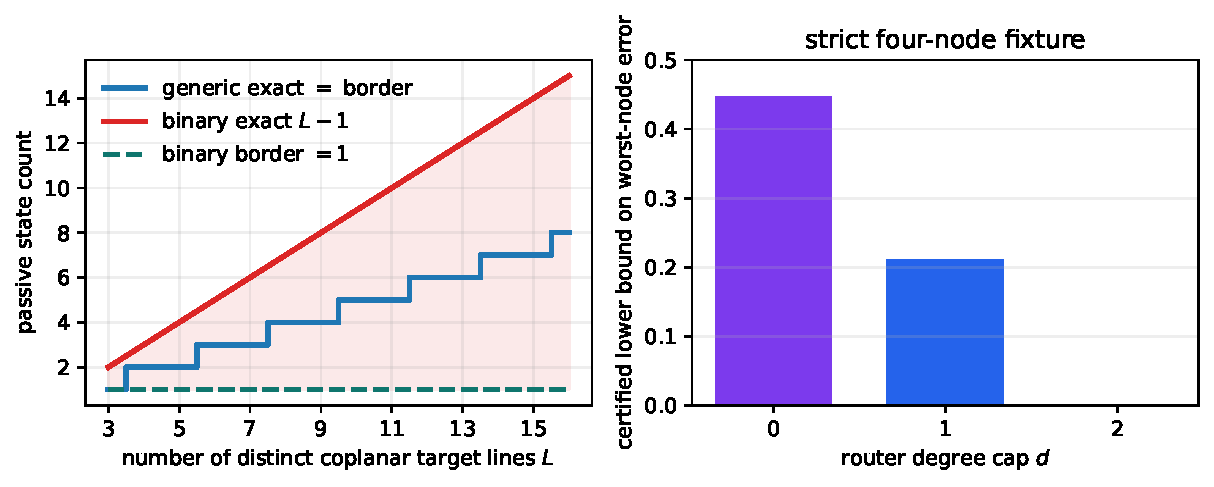
\includegraphics[width=0.98\linewidth]{figures/unbounded_detector_gap.pdf}
\caption{Left: generic exact/border memory and the binary $1+(L-1)$ split,
whose exact memory is $L-1$ while its border memory remains one; the shaded
exact-to-border gap is unbounded.  Right: exact certified worst-node
chordal-error barriers for the strict four-node fixture.  Degree two attains
zero error, whereas degrees zero and one remain quantitatively separated.}
\label{fig:gap}
\end{figure}

\section{The complete four-line phase diagram}

For four ordered distinct nodes, write
\[
 [z_1,z_2;z_3,z_4]
 =\frac{(z_1-z_3)(z_2-z_4)}{(z_1-z_4)(z_2-z_3)}
\]
with the usual projective conventions at infinity.  The order matters because
each frequency is paired with a specified target.
The projective classification below is classical/elementary; our claim is its
exact consequence for square passive rational-inner routers.

\begin{theorem}[Four-line classification]\label{thm:four}
For four target lines in one two-plane, the exact passive memory is
\begin{equation}\label{eq:four}
d_{\min}=\begin{cases}
0,&\text{all four targets coincide},\\
1,&\text{all four are distinct and their ordered cross-ratio equals that of the nodes},\\
3,&\text{the target multiplicities are }3+1,\\
2,&\text{in every remaining case.}
\end{cases}
\end{equation}
\end{theorem}

\begin{proof}
A nonconstant degree-one map is a projective bijection, so it sends the four
nodes to four distinct targets and preserves their ordered cross-ratio.  These
conditions are also sufficient by the uniqueness of a projective map through
three ordered points.

If three nodes share a target and the fourth does not, a nonconstant map of
degree at most two cannot work because every fiber has at most two distinct
points.  Polynomial interpolation gives the universal upper bound three.

It remains to show degree at most two in all other nonconstant cases.  For four
distinct targets with mismatched cross-ratio, normalize domain and target triples
to $(0,\infty,1)$, leaving $s\mapsto t$ with $s\ne t$.  Then
\[
 R(z)=z(az+b),\qquad
 a=\frac{t-s}{s(s-1)},\quad b=1-a
\]
has degree two and realizes the data.  For multiplicities $2+2$, after choosing
a finite chart use
\[
 R(z)=c\frac{(z-z_1)(z-z_2)}{(z-z_3)(z-z_4)}.
\]
For $2+1+1$, normalize the repeated nodes to $0,\infty$, the other nodes to
$1,s$, and the targets to $\infty,\infty,0,1$.  Choose
$a\notin\{0,1,s\}$ and set
\[
 q(z)=z,\qquad p(z)=A(z-1)(z-a),\qquad
 A=\frac{s}{(s-1)(s-a)}.
\]
This is a coprime degree-two witness.  None of these cases is constant or
degree one, completing the lower bounds and the classification via
\cref{thm:planar}.
\end{proof}

\begin{example}[Strict exact and approximate detector failure]\label{ex:strict}
Take
\[
 (\zeta_1,\zeta_2,\zeta_3,\zeta_4)=(1,i,-1,-i),\qquad
 (Y_1,Y_2,Y_3,Y_4)=(0,1,\infty,2).
\]
The ordered cross-ratios are $2$ and $1/2$, respectively.  Hence
$d_{\min}=2$, while both constant lower bounds equal one.  An exact witness is
\[
 p(z)=-\frac{(z-1)(3z-i)}2,\qquad q(z)=z+1,
 \qquad \Res(p,q)=-3-i\ne0.
\]
It takes the four requested projective values exactly.

There is also a finite approximation gap below degree two.  Normalize the four
target representatives to unit norm.  For $d=1$, exact arithmetic gives
\[
G_1=M_1^*M_1=
\begin{pmatrix}
17/10&1+3i/10&-9/10&-i/10\\
1-3i/10&17/10&i/10&-9/10\\
-9/10&-i/10&23/10&-1-3i/10\\
i/10&-9/10&-1+3i/10&23/10
\end{pmatrix}.
\]
The leading principal minors of $G_1-\frac38I$ are
\[
 \frac{53}{40},\quad\frac{213}{320},\quad
 \frac{637}{2560},\quad\frac{213}{20480},
\]
all positive.  Sylvester's criterion yields $G_1\succ\frac38I$, and
Theorem~\ref{thm:approx} therefore forces
\[
 \max_i\operatorname{dist}_{\rm ch}(S(\zeta_i)X,Y_i)
 >\sqrt{\frac{3}{67}}\approx0.2116
\]
for every router with at most one state.  Likewise,
$G_0-I\succ0$ gives the degree-zero barrier $1/\sqrt5\approx0.4472$.
The degree-two witness above attains zero, producing a certified finite-error
staircase rather than only an exact degree jump.
\end{example}

\section{Delay price and reproducibility}

For a differentiable lossless boundary response, define the Wigner--Smith
matrix
\[
                  Q(\theta)=-iS(e^{i\theta})^*
                             \frac{\dd}{\dd\theta}S(e^{i\theta}).
\]
Jacobi's formula gives
$\operatorname{tr}(S^{-1}\partial_\theta S)=\partial_\theta\log\det S$.
Together with Potapov's factorization and winding count, this gives
\[
             \int_0^{2\pi}\operatorname{tr}Q(\theta)\dd\theta
             =2\pi\,\mcdeg S
\]
for finite rational-inner $S$ \cite{Wigner1955,Smith1960}.  Combining it with
\cref{thm:global,thm:block} yields an exact action law.

\begin{corollary}[Optimal integrated delay]\label{cor:delay}
For every line-routing table, and every block-subspace incidence table,
\[
 \inf_S\int_0^{2\pi}\operatorname{tr}Q(\theta)\dd\theta=2\pi d_{\min}.
\]
The projective lossless completion attains the infimum.
\end{corollary}

The computational artifact uses exact arithmetic over $\mathbb Q(i)$.  It
checks the strict witness in Example~\ref{ex:strict}; exact representatives of the
constant, cross-ratio-compatible, $2+2$, $2+1+1$, and $3+1$ strata;
the normalized Gram matrices and Sylvester coercivity certificates behind the
degree-zero and degree-one approximation barriers; the exact two-target
zero-memory formulas and their sharp-collision ratios at four rational
parameters;
the explicit nonattained $E_1=0$ degeneration at four rational values of
$\varepsilon$;
full-column-rank exclusions below the
generic threshold; coprime threshold witnesses for every $3\le L\le16$; and
every nontrivial binary occupancy split through $L=16$ (119 exact cases).
For every $3\le L\le16$ it additionally checks the complete binary
positive-error/nonattainment/exact phase partition and an explicit degree-one
degeneration of the $1+(L-1)$ family, whose exact-to-border ratio is $L-1$.
For all 119 binary tables it independently recomputes full column rank just
below $d_\partial$ and a nontrivial kernel at $d_\partial$, directly auditing
the polynomial-time rank formula rather than inferring it from occupancies.
The frozen validator recomputes the content hash and checks declared coverage,
phase degrees, ranks, and bounds.  In CI the producer is replayed from scratch
and its byte-identical JSON is compared with the frozen record; this replay is
the algebraic check of cross-ratios, witness values, gcds, and resultants.
These calculations
audit examples and certificates; they are not substitutes for the proofs.

\begin{limitation}[Exact scope]
The global theorem assumes distinct frequency nodes, one input line, free
endpoint phase, and square finite rational-inner competitors.  Repeated nodes
require confluent jets.  The block theorem assumes a literal orthogonal direct
sum of bands; overlapping target subspaces require a different arrangement
law.  Fixed endpoint frames, prescribed remaining columns, lossy or active
architectures, and numerical values of the positive minimax errors beyond
degree zero are not claimed.  The perturbation theorem is only as meaningful
as its calibrated operator-norm model.  The high-delay theorem concerns
differentiation with respect to the dimensionless phase $\theta$; it is not a
theorem about resonator quality factor, stored energy, linewidth, or
fabrication cost.
\end{limitation}

\begin{limitation}[Priority scope]
Minimal scalar, vector, matrix, and tangential rational interpolation;
unattainable points and common factors; generic rational-curve dimension
counts; cross-ratios and fiber multiplicity; Fej\'er--Riesz factorization;
rectangular lossless realization, all-pass completion, and Potapov
factorization all predate this work
\cite{AntoulasEtAl1990,Ravi1997,BultheelVanBarel1990,Glader2008,
CortadellasUnattainable2018,BallKim1994,AlpayJorgensenLewkowicz2016}.
The Poisson-kernel group-delay formula and the divergent peak produced by a
Blaschke zero approaching $\T$ are classical as well.  What is claimed here is
that the projective border law forces this degeneration along every
nonattained routing sequence.
We do not claim a new interpolation algorithm or completion theorem.  The
claimed contribution is their synthesis for this passive architecture: the
global conversion into state count \eqref{eq:global}, the full-support block specialization
\eqref{eq:block}, the rank/error and deletion identities
\eqref{eq:rank-border}--\eqref{eq:delete}, the exact maximum/minimum split
between multiband exact and border memory, and the resonant trichotomy of
Theorem~\ref{thm:highq}.  The planar cap, binary, and cross-ratio results are
explicit strata and audit fixtures, not claims of priority for their classical
projective ingredients.
\end{limitation}

\paragraph{AI assistance disclosure.}
AI tools assisted with literature discovery, symbolic fixture generation,
code review, and language editing.  The author selected the claims, checked
the proofs and exact certificates, and takes responsibility for the content.

\paragraph{Reproducibility record.}
The accompanying archive contains the manuscript source, the planar exact
producer and independent validator, a separate rational-arithmetic verifier
for the block-subspace laws, the frozen JSON objects, and a hash manifest.  The
archive is tested after extraction; the validators do not import each other's
implementation.  The source base is commit
\nolinkurl{b2a7f3268de19683573325c5a63d4ce0030ed955}.  The frozen global and
planar certificate hashes are, respectively,
\nolinkurl{ecfa47a4585bb646716888b93cc0ca4fca6fc2c33c5373786790c6d010af210a}
and
\nolinkurl{09e3aa7dc2b2a80ce2222bae0a4a85357d0d36d09e257595b992ceb900db5c47}.
From the extracted archive the fail-closed replay is
\begin{quote}\small\ttfamily
python verification/verify\_global\_projective\_memory.py\\
\hspace*{1em}--check results/global\_projective\_memory/certificate.json\\
python verification/verify\_planar\_projective\_memory.py
\end{quote}
The
archive is distributed beside the PDF as
\texttt{Projective\_Memory\_Reproducibility.zip}; its final SHA-256 is recorded
in the companion submission sheet and detached manifest, avoiding a
self-referential archive hash inside the archive itself.

\section{Conclusion}

The exact state count of every finite line-routing table is the degree of one
projective curve in the actual target span.  This global identity replaces the
former collection of direct-sum and coplanar strata by a single invariant.
For block-subspace architectures, full-support Lagrange kernels give every
nongeneric exact degree, while generic codimensions yield a closed design law.
The closure problem is different: exact memory takes the most expensive band,
whereas border memory can survive in the cheapest, producing an arbitrarily
large separation already for scalar occupancies.

The incidence matrix makes this geometry falsifiable.  Full column rank gives
a calibrated positive chordal-error floor; first rank loss gives the exact
zero-infimum boundary; base-point deletion explains every missing record.
Most importantly, zero but unattained error is not free approximation.  A
bounded peak Wigner--Smith delay makes the fixed-degree lossless family compact,
so the nonattained phase can approach zero only by driving a Potapov zero to the
unit circle and creating a divergent delay peak.  Passive line routing therefore
has three operationally distinct phases: robust error, singular high-delay
approximation, and exact finite-delay realization.  The explicit planar cap,
binary occupancy, and four-node cross-ratio theorems show how the global laws
resolve the first collision strata without concealing their classical origins.

\clearpage
\begin{multicols}{2}
\bibliographystyle{unsrt}
\bibliography{global_references}
\end{multicols}
\end{document}
